\documentclass[10pt, draft]{book}


\usepackage[latin1]{inputenc}
\usepackage[T1]{fontenc}
\usepackage[italian]{babel}
\usepackage{a4wide}
\usepackage{makeidx}
\usepackage{url}
\usepackage{multicol}
\usepackage{amsthm}
\usepackage{colortbl}
\usepackage{amssymb}
\usepackage{synttree}
\usepackage{proof}


\newtheorem{teorema}{Teorema}
\newtheorem{proposizione}{Proposizione}
\newtheorem{corollario}{Corollario}
\newtheorem{definizione}{Definizione}
\newtheorem{osservazione}{Osservazione}
\newtheorem{notazione}{Notazione}
\newtheorem{lemma}{Lemma}
\newtheorem{esempio}{Esempio}
\newtheorem{dimostrazione}{Dimostrazione}

\title{Struttura del backend\\[2mm]{\small\emph{Anno Accademico 2010-2011}}\\[4mm]}
\author{\Nome\ \Cognome}

\newcommand{\Cognome}{Viscomi}
\newcommand{\Nome}{Federico}



\makeindex

\begin{document}

\maketitle

\tableofcontents

\chapter{Struttura del backend}
La figura 1 descrive la struttura composita di una certa porzione di Cupido. I

\begin{center}
  \begin{figure}[ht]
    \begin{center}
      \resizebox{\columnwidth}{!}{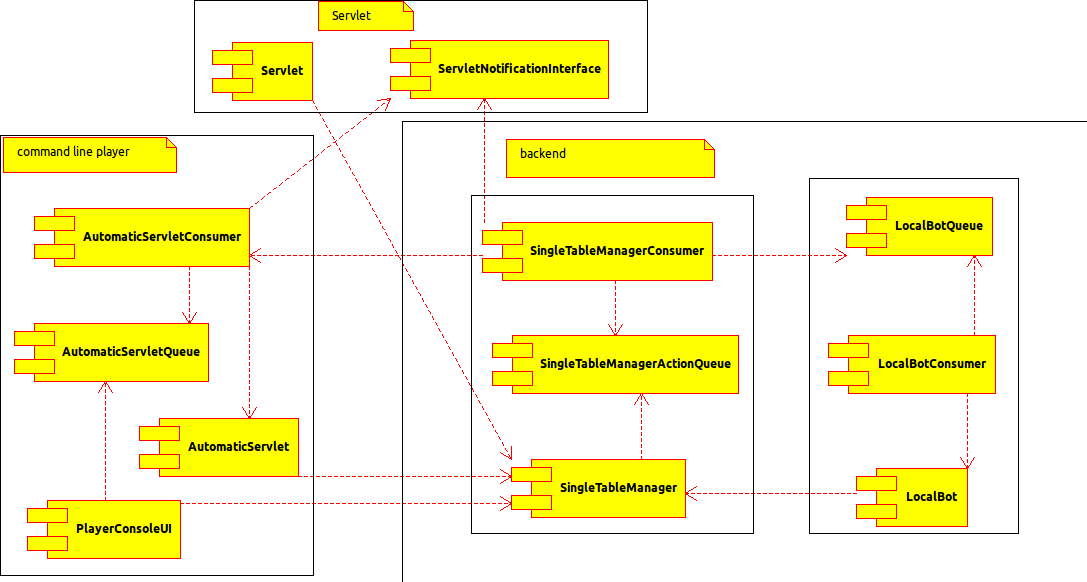
\includegraphics{backend_composit_structure.png}}
    \end{center}
    \caption{struttura composita di una parte di cupido}
    \label{fig:example}
  \end{figure}
\end{center}

\printindex

\end{document}
